%!TEX root=bare_conf.tex
\section{Evaluation}\label{sec:evaluation}

In general, this paper investigates the following research questions to evaluate PML\_Checker:
\begin{description}
\item[RQ1:] How does our approach perform under the real-world repositories and public benchmarks? 
\item[RQ2:] How does our approach perform in terms of effectiveness analysis for complex control flows? 
\item[RQ3:] How does our approach perform in terms of effectiveness analysis for complex data types? 
\end{description}

\subsection{RQ1: Performance on real-world repositories and public benchmarks}

%The first research question is to compare the accuracy achieved by the four approaches, and the run-time recorded by the corresponding $4$ tools in terms of open benchmarks. There are two experiments.

\subsubsection{Accuracy Analysis}

\ 

This section includes two-part experiments: experiment on large amount code (SPEC CPU $2000$ and SIR), experiment on small amount code (test cases from SARD).

Table~\ref{tab:3} shows the test results on SPEC CPU $2000$ and Table~\ref{tab:4} shows the test results on SIR. Compare PML\_Checker with other three tools, we have the following observations. 

First, calculate the \textit{FP} in Table~\ref{tab:3}. \textit{FP}(CppCheck) $\approx$ 11\%, \textit{FP}(Splint) = 44\%, \textit{FP}(RL\_Detector) = 9\%, \textit{FP}(PML\_Checker) = 13\%. Similarly, in Table~\ref{tab:5}, \textit{FP}(CppCheck) = 19\%, \textit{FP}(Splint) = 0.30\%, \textit{FP}(RL\_Detector) = 8\%, \textit{FP}(PML\_Checker) = 18\%.
In the view of \textit{TW} from Table~\ref{tab:3} and Table~\ref{tab:4}, Splint reports most bugs, and PML\_Checker ranks second, while CppCheck reports the least bugs. However, in the view of \textit{FP}, the \textit{FP} of Splint is highest, and the \textit{FP} of the other three tools are acceptable.

Second, this paper analyzes the effectiveness of the PML\_Checker by comparing the MLF of test results. Test results from Table~\ref{tab:3} can be converted into MLF of test results by constructing a matrix. Specifically, the results from Table~\ref{tab:4} can be abstracted to a sparse matrix consists of $15$ quaternions. This paper compresses this matrix by removing all the rows that test results are zero, and a row in the matrix corresponds to a row in the table of test results. The final matrix $D_1$ is as follows.

\begin{table}[!h]
\newcommand{\tabincell}[2]{\begin{tabular}{@{}#1@{}}#2\end{tabular}}
\centering
\setlength{\abovecaptionskip}{0pt}%    
\setlength{\belowcaptionskip}{10pt}%
\caption{Test results on SPEC CPU $2000$}\label{tab:3}
\centering
\begin{tabular}{|c|c|c|c|c|c|c|c|c|c|}
\hline
\multirow{2}{*}{\textbf{Program}}& \multirow{2}{*}{\tabincell{c}{\textbf{Size}\\\textbf{(Kloc)}}} & \multicolumn{2}{|c|}{\textbf\small{CppCheck}} & \multicolumn{2}{|c|}{\textbf\small{Splint}} &          \multicolumn{2}{|c|}{\textbf\small{RLDetector}} & \multicolumn{2}{|c|}{\textbf\small{PMLChecker}}\\
\cline{3-10}
 &  & \textbf\small{TW} & \textbf\small{NF} & \textbf\small{TW} & \textbf\small{NF} & \textbf\small{TW} &   \textbf\small{NF} & \textbf\small{TW} & \textbf\small{NF}\\
\hline
gzip       & 7.8    & 1  & 1 & 1	& 1   & 1   & 1  & 3  & 1\\
\hline
vpr        & 17.0   & 0  & 0 & 0	 & 0   & 0  &	0  &	4   &1\\
\hline
gcc        & 205.8 & 1  & 0 & 46 & 24 & 35 &	0  & 22 & 1\\
\hline
mesa     & 49.7   & 1  & 0 & 9	 & 5	   & 4  & 2  & 17 & 5\\
\hline
art         & 1.3     & 1  & 0 &0   & 0	   & 1  &	0   & 3  & 0\\
\hline
mcf        & 1.9     & 0  & 0 & 5  &  2  & 0   & 0  & 1  & 1\\
\hline
equake   & 1.5     & 0  & 0 & 0	 & 0   &	0  & 0   & 8  & 0\\
\hline
crafty     & 18.9   & 0	 & 0	 & 0	 & 0	  & 0   & 0   & 0   & 0\\
\hline
ammp    & 13.3   & 12 & 0 & 22 & 4  & 	20 & 0  & 22 & 2\\
\hline
parser    & 10.9   & 0	 & 0	 & 0	   &0  & 0    & 0  & 0  & 0\\
\hline
perlbmk & 58.2   & 2   & 1	 & 0	   & 0  &	4   & 1  & 2  & 0\\
\hline
gap        & 59.5   &  0 & 0 & 0    & 	0  &	0   & 0   & 0	& 0\\
\hline
vortex    & 52.7    & 0	 & 0	 & 0	   & 0  &	0   & 0   & 0	& 0\\
\hline 
bzip2     & 4.6      & 1 & 0	 & 2	   & 1  &	0   & 0   & 1	& 0\\
\hline
twolf     & 19.7     & 0 & 0	 & 0	   & 0  &	0   & 0   & 0	& 0\\
\hline
Total     & 581      & 19 & 2 & 85 &	37 & 65 & 6	& 83 & 11\\
\hline
\end{tabular}
\end{table}

\begin{table}[!h]
\newcommand{\tabincell}[2]{\begin{tabular}{@{}#1@{}}#2\end{tabular}}
\centering
\setlength{\abovecaptionskip}{0pt}%    
\setlength{\belowcaptionskip}{10pt}%
\caption{Test results on SIR}\label{tab:4}
\centering
\begin{tabular}{|c|c|c|c|c|c|c|c|c|c|}
\hline
\multirow{2}{*}{\textbf{Program}}& \multirow{2}{*}{\tabincell{c}{\textbf{Size}\\\textbf{(Kloc)}}} & \multicolumn{2}{|c|}{\textbf\small{CppCheck}} & \multicolumn{2}{|c|}{\textbf\small{Splint}} &           \multicolumn{2}{|c|}{\textbf\small{RLDetector}} & \multicolumn{2}{|c|}{\textbf\small{PMLChecker}}\\
\cline{3-10}
 & & \textbf\small{TW} & \textbf\small{NF} & \textbf\small{TW} & \textbf\small{NF} & \textbf\small{TW} & \textbf\small{NF} & \textbf\small{TW} & \textbf\small{NF}\\
\hline
bash       & 59.8 &7	&1	  & 15  & 3  & 3	 & 0   & 17  & 2\\
\hline
flex	       & 10.5  & 1	& 0	  & 2    & 1  & 2	 & 1	   & 2   & 1\\
\hline
grep	 & 10.1 & 3	& 1	  & 0    & 0  & 0	 & 0	   & 2   & 0\\
\hline
gzip	       & 5.7   & 0	& 0	  & 0    & 0  & 0	 & 0	   & 0   & 0\\
\hline
make	 & 35.5 &1	& 0	  & 0    & 0  & 0	 & 0	   & 1   & 0\\
\hline
print	 & 0.7   &  0	& 0	  & 0    & 0  & 0	 & 0	   & 0   & 0\\
\hline
print2	 & 0.6   & 0	& 0	  & 0    & 0  & 0	 & 0   &	0   & 0\\
\hline
replace    & 0.6   & 0	& 0	  & 0    & 0  & 0	 & 0	   & 0   & 0\\
\hline
schedule  & 0.4	& 0	& 0	  & 5    & 2  & 0	 & 0	   & 2   & 0\\
\hline
schedule2 & 0.4	& 0	& 0    & 3    & 0  & 0	 & 0	   & 2   & 1\\
\hline
sed	        & 14.4	& 4	& 2    &	0   & 0  & 0	 & 0	   & 3   & 0\\
\hline
space	 & 6.2	& 2	& 0	   & 0   & 0  & 0	 & 0	   & 1   & 1\\
\hline
tcas	       & 0.2	& 0	& 0    &	0   & 0  & 0	 & 0    & 0   & 0\\
\hline
totinfo	 & 0.6	& 0  & 0	   & 0    & 0  & 0	 & 0	   & 0   & 0\\
\hline
vim        & 122.2	& 3	& 0	   & 12  & 5  & 8	 & 0	   & 4   & 1\\
\hline
Total	 & 267.9	 & 21&4	   & 37  & 11 & 13 & 1   & 34  & 6\\
\hline
\end{tabular}
\end{table}

\[
\scriptsize
D_1=\left[
\begin{array}{cccccccccc}
0 & 0 & 35 & 2 & 1 & 0 & 0 & 20 & 3 & 0\\
0 & 0 & 1  &  1 & 1 & 0 & 0 & 12 & 1 & 1\\
0 & 0 & 22 & 4 & 0 & 3 & 0 & 18 & 0 & 1 \\
2 & 3 & 21 & 12 & 3& 0 & 8 & 20 & 2 & 1  
\end{array}
\right]^{T}
\]

Similarly, $D_2$ is the matrix abstracted from Table~\ref{tab:4}, and $D_2$ is shown as follow:
\[
\scriptsize
D_2=\left[
\begin{array}{ccccccccc}
3 & 1 & 0 & 0 & 0 & 0 & 0 & 0 & 8 \\
6 & 1 & 2 &  1 & 0 & 0 & 2 & 2 & 3\\
12 & 1 & 0 & 0 & 3 & 3 & 0 & 0 & 7 \\
15 & 1 & 2& 1 & 2 & 1 & 3 & 0 & 3  
\end{array}
\right]^{T}
\]

\begin{figure}[!h]
\center
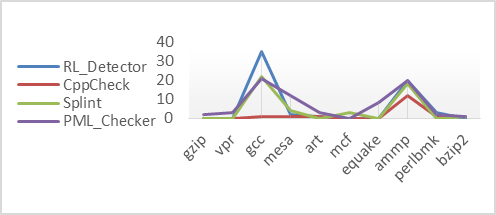
\includegraphics[width=0.45\textwidth]{figure/fig8-fig12/fig10}
\caption{The MLF of each tool on SPEC CPU 2000}
\label{fig:10}
\end{figure}

\begin{figure}[!h]
\center
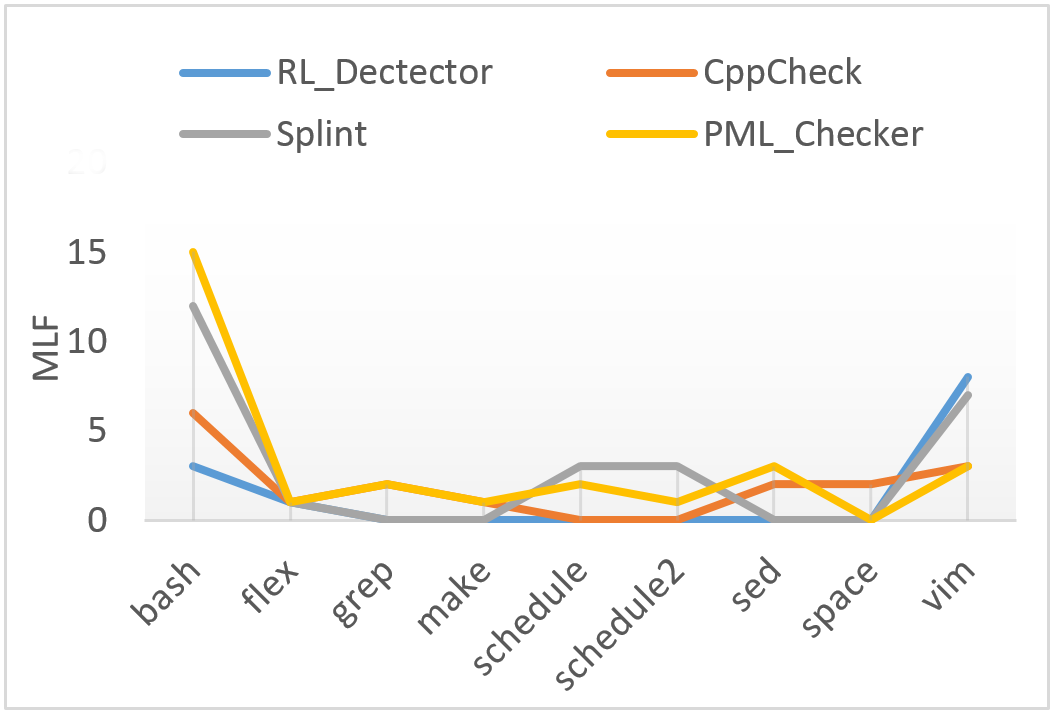
\includegraphics[width=0.45\textwidth]{figure/fig8-fig12/fig11}
\caption{The MLF of each tool on SIR}
\label{fig:11}
\end{figure}

In Fig.~\ref{fig:10}, the abscissa shows the name of the program corresponding to each row in the matrix, and the ordinate shows the value of corresponding MLF. This figure displays the number of memory leaks confirmed by manually checking, among the test results on the $15$ programs from SPEC CPU $2000$. We conclude from Fig.~\ref{fig:10} that PML\_Checker has a good detection result on the test sets relatively. There is a big difference from test results for \textit{gcc}. \textit{gcc} is larger than others in size. Therefore, we deduce that the scalability of the PML\_Checker and CppCheck for large scale test objects needs to be improved. 

In Fig.~\ref{fig:11}, due to the smaller amount code of SIR comparing to SPEC CPU 2000 and fewer \textit{TW} of each tool, the advantage of PML\_Checker is not obvious. But the analysis results between the two benchmarks are generally consistent. By testing on SPEC CPU $2000$ and SIR, PML\_Checker shows a good performance in testing memory leak.

Table~\ref{tab:5} shows the test results on $40$ test cases from SARD. Compare PML\_Checker with other three Tools, we have the following observations.
First, calculate the \textit{NP} of the test results of $20$ test cases with memory errors marked ``bad", and the \textit{FP} of the test results of $20$ test cases without memory errors which corresponding to the ``bad" cases marked ``good". \textit{NP}(RL\_Detector) = 70\%, \textit{FP}(RL\_Detector) = 0. \textit{NP}(CppCheck) = 50\%, \textit{FP}(CppCheck) = 0. \textit{NP}(Splint) = 80\%, \textit{FP}(Splint) = 5\%. \textit{NP}(PML\_Checker) = 30\%,  \textit{FP}(PML\_Checker) = 0. The \textit{FP} of PML\_Checker is the lowest among the four tools. For the analysis of \textit{FP}, there are no false positives in the results of RL\_Detector, CppCheck and PML\_Checker. While Splint reports a false positive. This experiment fails to compare the \textit{FP} due to the small size of program, but the test results on \textit{NP} reflects the accuracy of PML\_Checker in detecting memory leaks.
\begin{table}[!h]
\newcommand{\tabincell}[2]{\begin{tabular}{@{}#1@{}}#2\end{tabular}}
\center
\caption{Test results on SARD test cases}\label{tab:5}
\begin{tabular}{|c|c|c|c|c|}
\hline
\textbf{Cases} &       \tabincell{c}{\textbf{CppCheck}\\\textbf{(TW)}} &           \tabincell{c}{\textbf{Splint}\\\textbf{(TW)}} &               \tabincell{c}{\textbf{RLDetector}\\\textbf{(TW)}} & \tabincell{c}{\textbf{PMLChecker}\\\textbf{(TW)}}\\
\hline
bad  &10 & 4 & 6 & 14\\
\hline
good  & 0 & 1 &	0 &	0\\
\hline
\end{tabular}
\end{table}

%\begin{figure}[!h]
%\center
%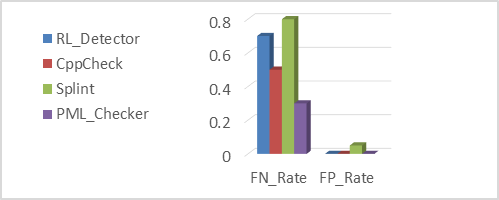
\includegraphics[width=0.45\textwidth]{figure/fig8-fig12/fig12}
%\caption{The bar chart of test results}
%\label{fig:12}
%\end{figure}
\subsubsection{Efficiency Analysis} 

\ 

Considering CppCheck, RL\_Detector and PML\_Checker all use symbolic execution, it is necessary to verify whether our approach affects the efficiency. This experiment chooses SPEC CPU $2000$ as the test object due to its large amount of code and large number of files, and analyzes the \textit{RunTime} of the three tools. 

Table~\ref{tab:6} lists the \textit{RunTime} of CppCheck, RL\_Detector and PML\_Checker. By comparing the \textit{RunTime} of these three tools, we conclude that the performance of RL\_Detector and PML\_Checker is better than CppCheck in \textit{RunTime}, and our approach does not affect the efficiency of PML\_Checker.

\begin{table}[!h]
\newcommand{\tabincell}[2]{\begin{tabular}{@{}#1@{}}#2\end{tabular}}
\centering
\caption{RunTime on SPEC CPU $2000$}\label{tab:6}
\centering
\begin{tabular}{|c|c|c|c|c|}
\hline
\multirow{2}{*}{\textbf{Program}}& \multirow{2}{*}{\tabincell{c}{\textbf{Size}\\\textbf{(Kloc)}}}&  \multicolumn{3}{|c|}{\textbf{RunTime(s)}}\\\cline{3-5}

& &   \textbf{CppCheck} &      \textbf{RLDetector}&  \textbf{PMLChecker}\\
\hline
gzip       & 7.8    & 5.3  & 4.5 & 3.2\\
\hline
vpr        & 17.0   & 10.0  & 7.5 & 7.6\\
\hline
gcc        & 205.8 & 167.7  & 48.3 & 41.0 \\
\hline
mesa     & 49.7   & 51.0  & 33.1 & 34.8\\
\hline
art         & 1.3     & 0.3  & 0.9 & 0.4\\
\hline
mcf        & 1.9     & 1.0  & 4.0 & 3.7\\
\hline
equake   & 1.5     & 0.2  & 1.0 & 0.4\\
\hline
crafty     & 18.9   & 27.3	 & 14.2	 & 13.3\\
\hline
ammp    & 13.3   & 7.4 & 10.3 & 10.0\\
\hline
parser    & 10.9   & 4.0	 & 6.7	 & 5.1\\
\hline
perlbmk & 58.2   & 123.2   & 41.3	 & 39.0\\
\hline
gap        & 59.5   &  29.0 & 20.9 & 20.0\\
\hline
vortex    & 52.7    & 73.2	 & 30.1	 & 26.7\\
\hline 
bzip2     & 4.6      & 2.0 & 0.6	 & 1.5\\
\hline
twolf     & 19.7     & 11.0 & 23.7	 & 24.0\\
\hline
Total     & 581.0    & 512.6 & 247.1 & 230.7\\
\hline
\end{tabular}
\end{table}

\subsection{RQ2: Effectiveness Analysis of Complex Control Flows}

\begin{table}[!h]
\center
\caption{Test results on complex control flows}\label{tab:7}
\begin{tabular}{|c|c|c|c|c|}
\hline
\textbf{Cases}  & \textbf{CppCheck} & \textbf{Splint} & \textbf{RLDetector} & \textbf{PMLChecker}\\
\hline
branch1	 &$\surd$ & $\times$ & $\surd$ & $\surd$\\
\hline
branch2    & $\surd$ & $\surd$ & $\surd$ & $\surd$\\
\hline
loop1	 &$\times$ &	$\times$ & $\surd$ & $\surd$\\
\hline
loop2    & $\surd$ &$\times$ & $\surd$ & $\surd$\\
\hline
chainBranch1 & $\times$ & $\times$ & $\surd$ & $\surd$\\
\hline
chainBranch2 &	$\times$	& $\times$ & $\surd$ & $\surd$\\
\hline
chainLoop1	 & $\surd$ & $\surd$ & $\times$ & $\surd$\\
\hline
chainLoop2	 & $\surd$& $\surd$ & $\times$ & $\surd$\\
\hline
nestingBranch	 & $\times$ & $\times$ & $\surd$ & $\surd$\\
\hline
nestingLoop& $\times$ & $\times$ & $\surd$ & $\surd$\\
\hline
\end{tabular}
\end{table}

%\begin{figure}
%\center
%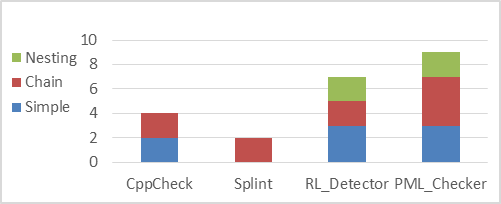
\includegraphics[width=0.45\textwidth]{figure/fig8-fig12/fig8}
%\caption{Description of memory leaks reasons}
%\label{fig:8}
%\end{figure}

%First, all the $4$ tools did not detect the memory leak in C\_case2, because the memory leaks in C\_case2 are caused by allocating memory blocks in conditional branches. In this case, the program will be compiled failed, because the pointer pointing to memory blocks is not found during the execution of function ``free()". Therefore, this type of test case is often ignored in static analysis.

%First, we calculated the \textit{NP} of the test results. In details, the false negative rate of CppCheck test results, that is \textit{NP}(CppCheck) is 5/9 $\approx$ 0.56. In the same way, \textit{NP}(Splint) = 0.78, \textit{NP}(RL\_Detector) = 0.22, while \textit{NP}(PML\_Checker) = 0. For the reason that the analysis method of PML\_Checker is based on the complex control flow, the results of PML\_Checker covered all the test cases about complex control flow in this experiment. In other words, the false negative rate of the CFG projection approach is lower than other approaches for detecting memory leaks in complex control flow, which reflects the effectiveness of this approach for complex control flow.
Table~\ref{tab:7} lists the test results on $10$ small programs. Comparing PML\_Checker to other threetools, we have the following observations.
First, calculate the \textit{NP} of the test results. \textit{NP}(CppCheck) = 50\%, \textit{NP}(Splint) = 70\%, \textit{NP}(RL\_Detector) = 20\%, \textit{NP}(PML\_Checker) = 0. PML\_Checker covered all the test cases about complex control flows. In other words, the results reflect the effectiveness of PML\_Checker on complex control flows.
Second, regarding the comparison of the approaches. Obviously, our approach has advantage of complex-control-flow detection. The regular match based approach matches the source code with the vulnerabilities in the process of detection. This approach is not sensitive and inflexible to complex control flow. The style and notation based approach improves the software quality by improving the programming style, and discoves the potential bugs of program. However, this kind of analysis is not complete, so it has a high false negative rate. The approach by constructing resources streamlined slices only makes a simple assumption for allocation and deallocation of resources within loop bodies. It reduces the number of loops to 1 and treats the loops the same as branches. Therefore, this approach can not pass the test cases on the chain\_loop structure (chainLoop1 and chainLoop2) in the experiment. \\


\subsection{RQ2: Effectiveness Analysis of Complex Data Types}

\begin{table}[!h]
\center
\caption{Test results on complex data types}\label{tab:8}
\begin{tabular}{|c|c|c|c|c|}
\hline
\textbf{Cases}  & \textbf{CppCheck} & \textbf{Splint} & \textbf{RLDetector} & \textbf{PMLChecker}\\
\hline
array1	 &	$\surd$ & $\times$ & $\surd$ & $\surd$\\
\hline
array2  & $\times$ & $\times$ & $\times$ & $\times$ \\
\hline
array3	 & $\times$ &	$\times$ & $\times$ & $\surd$\\
\hline
list1 	& $\times$ &$\times$ & $\times$ & $\times$\\
\hline
list2	 & $\times$ & $\surd$ & $\times$ & $\surd$\\
\hline
list3	 &	$\times$	& $\surd$ & $\times$ & $\surd$\\
\hline
struct1	 & $\times$ & $\surd$ & $\times$ & $\surd$\\
\hline
struct2	 & $\times$ & $\surd$ & $\times$ & $\surd$\\
\hline
arrayStruct1	 & $\times$ & $\surd$ & $\surd$ & $\surd$\\
\hline
arrsyStruct2  & $\surd$ & $\surd$ & $\surd$& $\surd$\\
\hline
\end{tabular}
\end{table}

%\begin{figure}[!h]
%\center
%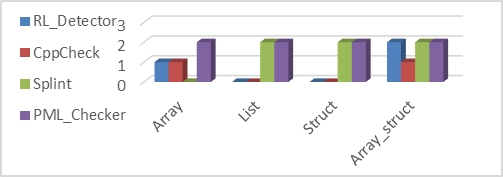
\includegraphics[width=0.45\textwidth]{figure/fig8-fig12/fig9}
%\caption{The leaks number of each data type}
%\label{fig:9}
%\end{figure}

%First, the common high NP shows us the accuracy of pointer alias analysis on complex data flow is relatively lower for all the tools.
Table~\ref{tab:8} lists the test results on $10$ small programs. Comparing our approach with other approaches, we have the following observations.
First, calculate the \textit{NP} of the test results. \textit{NP}(CppCheck) = 80\%, \textit{NP}(Splint) = 40\%, \textit{NP}(RL\_Detector) = 70\%, \textit{NP}(PML\_Checker) = 20\%. The results of Splint and PML\_Checker show a higher effectiveness. Splint has a high effectiveness because it mainly checks the specifications in programs, since it is sensitive to different data types. PML\_Checker shows a high effectiveness, because it simplifies the analysis for complex data types in the process of abstracting the control flows.
Second, comparing PML\_Checker to Splint, Splint reports memory leaks on the latter three data types (linked list, struct and array\_struct), except the memory leaks in an array. Due to the programs that are provided in this paper are in small scale and simple data relationships, PML\_Checker shows a little advantage compared with Splint. For the former approaches, that is CppCheck and RL\_Detector, there is a large space to improve in analyzing the complex data types.

\subsection{Summary}
From the above experimental results, we have the following main findings including advantages and limitations: 
\begin{itemize}
\item 
For the accuracy of detection, PMl\_Checker shows a lower false negative comparing to other three tools, while it shows a high false positive rate in real-world repositories (SPEC CPU $2000$ and SIR). Therefore, in the next step, more detailed data flow analysis are plan to be added into our approach.
\item 
For the complex control flows and complex data types analysis, PML\_Checker is better than the other three tools.
\item 
For the scalability of detection, our experiment needs to expand the range of detection. Specifically, it is possible to detect the large scale benchmarks with millions of code lines, or source code from some open-source software.
\end{itemize}
